\section{Introducción}

Este trabajo consistirá en analizar el funcionamiento de un amplificador real, para lo cual se deberá tener en cuanta las fuentes de error que están presentes en el mismo, lo que causa una desviación en la salida que deberá ser tenida en cuenta para el diseño de un sistema robusto.\\

Los errores que deberán ser tenido en cuenta para el análisis son los siguientes:\\

\textbf{Errores en DC.}
\begin{itemize}
    \item Error de offset de tensión $V_{os}$.\\
    \item Error de corriente de polarización $I_{os}$.\\
    \item Error por ganancia no infinita $Ad < \infty$.\\
    \item Error por RRMC no infinita $RRMC < \infty$.\\
\end{itemize}

\textbf{Errores en AC.}
\begin{itemize}
    \item Error Vectorial.\\
    \item Ancho de banda en pequeña señal.\\
    \item Ancho de banda en plena potencia.\\
\end{itemize}

Se hará un análisis teórico y simulaciones para corroborar lo obtenido.


\subsection{Objetivos}
    \begin{itemize}
        \item Aplicar el conocimiento teórico - práctico para analizar los errores acarreados en circuitos que hacen uso de amplificadores operacionales.\\
        \item Identificar las limitaciones respecto a la exactitud del respuesta ofrecida por el amplificador utilizado.\\
        \item Fortalecer el uso del simulador LtSpice e interpretar los resultados del mismo realizando las comparaciones correspondientes con los resultados te´oricos obtenidos.\\
    \end{itemize}

\newpage


\section{Sumador Inversor}
\subsection{Circuíto}
    \begin{figure}[ht]
    	\centering
    	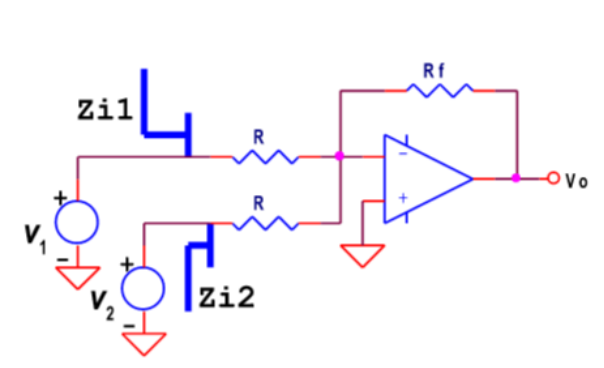
\includegraphics[height=5cm]{Imágenes/SumInv.png}
    	\caption{Circuíto a analizar}
    \end{figure}

\subsection{Requerimientos}
    Para desarrollar el trabajo, se deberá emplear el circuito propuesto, con el amplificador operacional LM324. Se deberá cumplir con las siguientes especificaciones establecidas:\\
    \begin{itemize}
        \item $V_{cc} = 10 [V]$ y $V_{ss} = -10 [V]$.\\
        \item $Av_{v1} = 30$ y $Av_{v2} = 30$.\\
        \item $R_{i} << Z_{i1}$ y $R_{i} << Z_{i2}$.\\
        \item Emplear resistencias menores a 10 [M$\Omega$].\\
    \end{itemize}

    \newpage


\section{Desarrollo}
\subsection{Ganancia Ideal}
Para obtener la ganancia ideal, debemos aplicar superposición, para esto:\\

\textbf{Pasivando V1}\\
$V_{o}|_{V1 = 0} = -\frac{R_{f}}{R}$\\

\textbf{Pasivando V2}\\
$V_{o}|_{V2 = 0} = -\frac{R_{f}}{R}$\\

\begin{center}
    \boxed{V_{o} = -\frac{R_{f}}{R} *(v_{1} + v_{2})}
\end{center}

\subsection{Errores en DC}
En esta sección se verán los errores en corriente contínua, para ello se modelará en cada caso una fuente de error colocada estratégicamente; Los errores son analizados de manera separada y luego por superposición sumado los efectos, esto evita cálculos extensos pero se ignoran las alinealidades que el sistema pudiese tener.\\

Se utilizará además la fórmula de \textbf{Blackman} y se suponen el resto de características del amplificador ideales a excepción de la cual debemos calcular el error.\\

Se procede a calcular la ganancia de lazo:\\

\begin{center}
    \boxed{T(s) = -Ad(s)*\frac{R}{R + 2*R_{f}}}
\end{center}

\subsubsection{Error de offset de tensión $V_{os}$.}
Se modela colocando en la entrada no inversora una fuente de tensión contínua de entrada, y de valor $V_{os}$.\\

\begin{center}
    \boxed{\frac{V_{o}}{V_{os}} = 1 + \frac{R_{f}}{R/2}}
\end{center}

\begin{center}
    \boxed{ V_{o} = (1 + \frac{R_{f}}{R/2}) * V_{os}}
\end{center}
\newpage
\subsubsection{Error de corrientes de polarización $I_{os}$}

\begin{center}
    \textbf{$I_{p+}$}\\
\end{center}

    En este caso no se generará una tensión en la entrada positiva del amplificador debido a esta corriente, ya que no se posee una resistencia en tal punto que levante una diferencia de potencial tal que sea amplificada.\\
    
\begin{center}
    \textbf{$I_{p-}$}\\
\end{center}

    $V_{o} = V_{-} * \frac{R + 2*R_{f}}{R}$\\
    
    \begin{center}
        \boxed{ V_{o} = -I_{p-}*\frac{R*R_{f}}{R + 2*R_{f}}*\frac{R + 2*R_{f}}{R} = -I_{p}*R_{f}}
    \end{center}


\subsubsection{Error por ganancia no infinita $Ad < \infty$.}
    Es posible definir la ganancia real de un amplificador operacional mediante la fórmula de blackman, mediante la siguiente expresión:

    \begin{center}
        \boxed{Av(s) = \frac{A_{vfi}}{ 1 - \frac{1}{T(s)}}}
    \end{center}

    Si la ganancia del amplificador tiende a infinito, entonces la ganancia será ideal, pero como no es infinita, entonces se puede definir un error como:\\

    \begin{center}
        \boxed{Av(s) = \frac{A_{vfi}}{ 1 - e_{g}}}
    \end{center}

     Por lo que:\\

    \begin{center}
        \boxed{\Delta V_{o} = e_{g}(0)*V_{dmax}}
    \end{center}

    pero $V_{dmax} = FS$, entonces:

    \begin{center}
        \boxed{\Delta V_{o} = e_{g}(0)*FS = \frac{FS}{T(0)}}
    \end{center}

    \newpage
\subsubsection{Error por RRMC no infinita $RRMC < \infty$.}
    Ya que la entrada no inversora está en masa, el error producido por la relación de rechazo en modo común es completamente despreciable, debido a que la tensión común es muy cercana a cero.
    
\subsection{Errores en AC}
    Para hacer el análisis en AC, se debe tener en cuenta ahora las variaciones de los componentes debido a la frencuencia, tomamos el amplificador operacional como un dispositivo de ún sólo polo, es decir de primer orden, con la siguiente función de transferencia:\\

    \begin{center}
        \boxed{A_{vf}(s) = \frac{A_{vf}(0)}{(1 + \frac{s}{\omega_{H}})}}
    \end{center}
    
\subsubsection{Error Vectorial.}
    Es definido como la diferencia vectorial entre la ganancia ideal y la real.
    \begin{center}
        \boxed{E_{v} = A_{vfi} - A_{vf}(s)}
    \end{center}

    Al ser un vector, es posible determinar mediante dos errores, error de ganancia o de módulo y error de fase.\\

    \textbf{Error de ganancia:} Diferencia entre los módulos de la ganancia real y ideal. Aplicando esto y normalizando:\\

    \begin{center}
        \boxed{e_{v} = |1| - |\frac{1}{1 + \frac{s}{\omega_{H}} }|}
    \end{center}

    \begin{center}
        \boxed{e_{v} = 1 -\frac{1}{\sqrt{1 + (\frac{\omega}{\omega_{H}})^2 }} }
    \end{center}

    \textbf{Error de Fase:} Diferencia entre las fases de la ganancia real y ideal:\\

    \begin{center}
        \boxed{\phi_{v} = -arctg(\frac{\omega}{\omega_{H}}) + \frac{\pi}{2}}
    \end{center}
    
\subsubsection{Ancho de banda en pequeña señal.}
    Al ser un sistema de primer orden, es definido como el punto donde la ganancia cae -3[dB] respecto a la banda de paso. Podemos aplicar el producto ganancia-Ancho de banda constante debido a este comportamiento de primer orden:\\

    $\omega_{H}*A_{vf} = 1*\omega_{T}$
    
    \begin{center}
        \boxed{\omega_{H} = \frac{\omega_{T}}{A_{vf}}}
    \end{center}
    
\subsubsection{Ancho de banda en plena potencia.}
    Es la máxima frecuencia que puede colocarse en el amplificador operacional, para que en su salida no se presente distorsión a su máxima potencia.\\

    \begin{center}
        \boxed{\omega_{HP} = \frac{SR}{V_{pp}}}
    \end{center}

    Donde, $V_{pp}$ es la tensión pico a pico máxima presentada en la entrada del amplificador.\\

\newpage

\section{LM324}
Desde la hoja de datos del Amplificador Operacional podemos determinar los siguientes parámetros típicos:\\
\begin{itemize}
    \item $V_{os} = 0.6 [mV]$.
    \item $RRMC = 80 [dB]$.
    \item $I_{os} = 0.5 [nA].$
    \item $I_{p} = 10 [nA].$
    \item $SR = 0.5 [V/uS].$
    \item $Ad0 = 100 [dB].$
    \item $f_T = 1 [MHz].$
\end{itemize}

\section{Caso de Estudio:$R_{i} = 50 \Omega$ }
Si tenemos una impedancia interna de la fuente de ese valor especificado, para no cargar a la misma, la impedancia de entrada deberá ser de al menos 10 veces mayor, esto es:\\

$R_{i} = 50 [\Omega] \xrightarrow{} Z_{i1,2} \ge 10*R_{i} $\\

$R \ge 500[\Omega] $\\

Si tomo que $R=1.8 [K\Omega]$, entonces:

$\frac{R_{f}}{R} = 30 \xrightarrow{} R_{f} = 54 [K\Omega]$.\\

\subsection{Errores DC}

\begin{itemize}
    \item $\Delta V_{o}|_{vos} = (1 + 2*\frac{R_f}{R})*V_{os} = 36.6 [mV].$\\
    \\
    Se procede a conectar una fuente de tension V5 de 0.6mV valor de Vos indicado por el fabricante a la entrada No Inversor y observar la salida del circuito y verificar que calculo hecho anteriormente es correcto.
    \begin{figure}[H]
    \centering
    \begin{minipage}{0.48\textwidth}
        \centering
        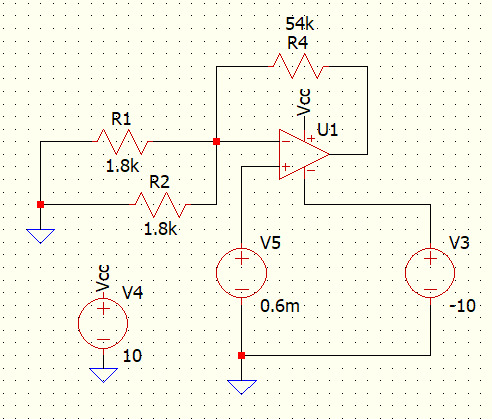
\includegraphics[height=5cm]{Imágenes/Simulaciones/Diagrama Vos 50.jpeg}
        \caption{Diagrama de Error Vos.}
        \label{fig:diagrama_vos}
    \end{minipage}
    \hfill
    \begin{minipage}{0.48\textwidth}
        \centering
        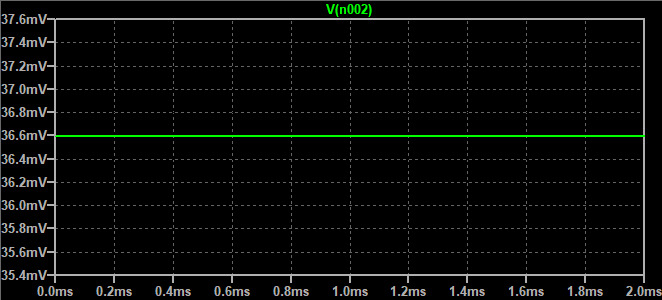
\includegraphics[height=5cm, width=8cm]{Imágenes/Simulaciones/vos 50.jpeg}
        \caption{Simulación del Error Vos.}
        \label{fig:simu_vos}
    \end{minipage}
\end{figure}
\newpage
    \item $\Delta V_{o}|_{Ios} = I_{os}.R_f = 0.54 [mV].$\\
    \\
    En cuanto al error por corrientes de polarización, no se puede simular exactamente, ya
que no se tiene una resistencia conectada al terminal no inversor, pero si se conecta una
fuente de corriente al terminal inversor, de modo de simular la Ip- planteada, se obtiene lo siguiente:
    \begin{figure}[H]
    \centering
    \begin{minipage}{0.48\textwidth}
        \centering
        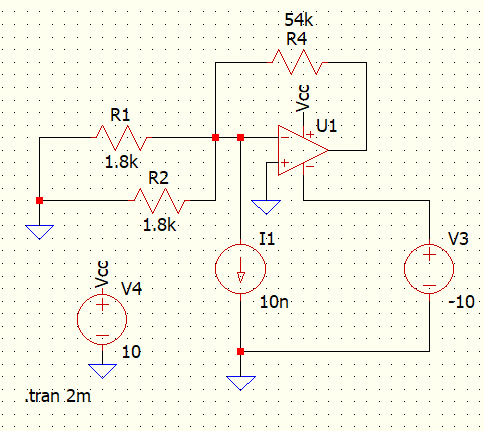
\includegraphics[height=5cm]{Imágenes/Simulaciones/ios 50 diagrama.jpeg}
        \caption{Diagrama de Error Ios.}
        \label{fig:diagrama_vos}
    \end{minipage}
    \hfill
    \begin{minipage}{0.48\textwidth}
        \centering
        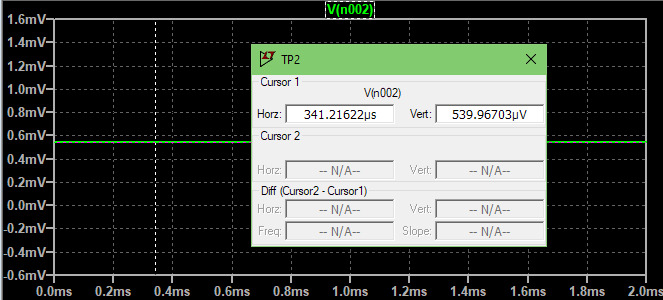
\includegraphics[height=5cm, width=8cm]{Imágenes/Simulaciones/ios 50.jpeg}
        \caption{Simulación del Error Ios.}
        \label{fig:simu_vos}
    \end{minipage}
\end{figure}
    \item $\Delta V_{o}|_{Ad < \infty} = \frac{FS}{To} = 6.1 [mV].$
    \item $\Delta V_{o}|_{RRMC < \infty} = 0 [mV].$
\end{itemize}

Por lo que el error total en contínua será de $\Delta Vo = 43.24 [mV].$

\subsection{Errores AC}
\textbf{Ancho de Banda de plena Potencia}.\\

$f_{HP} = \frac{SR}{2*\pi*V_{pp}} = 8 [KHz].$\\

\textbf{Ancho de Banda de pequeña Señal}.\\

$f_{HP} = k.f_T = \frac{R}{R+ 2*R_f}*f_t = 16.393 [KHz]$\\
\begin{figure}[ht]
    	\centering
    	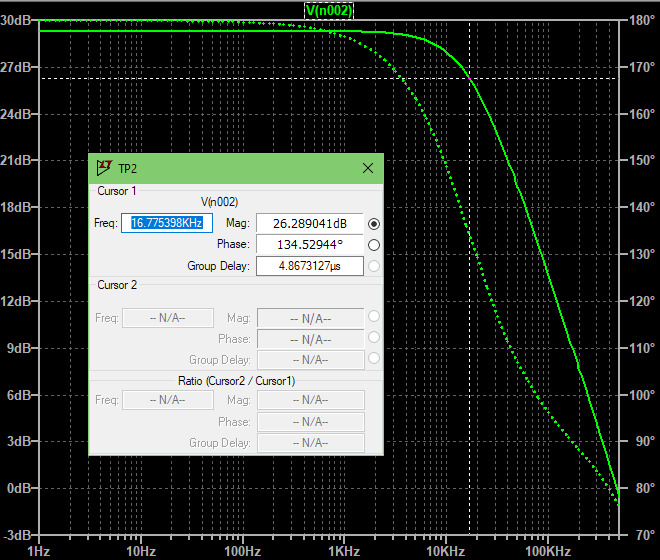
\includegraphics[height=5cm]{Imágenes/Simulaciones/bode 50.jpeg}
    	\caption{Diagrama de Bode Pequeña Señal}
    \end{figure}

\newpage
\textbf{Error Vectorial}.\\

    \begin{figure}[H]
    	\centering
    	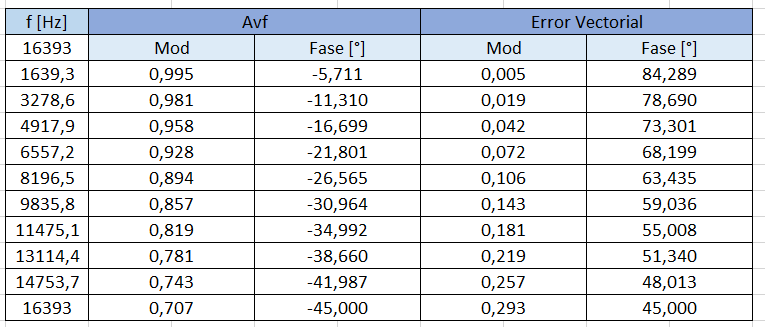
\includegraphics[height=5cm]{Imágenes/err1.png}
    	\caption{Error Vectorial}
    \end{figure}
\textbf{Slew Rate}\\
\\
Inyectamos un Señal cuadrada de 10V por V1 y conectando V2 a masa obtuvimos la pendiente de Slew Rate.\\


    \begin{figure}[H]
    	\centering
    	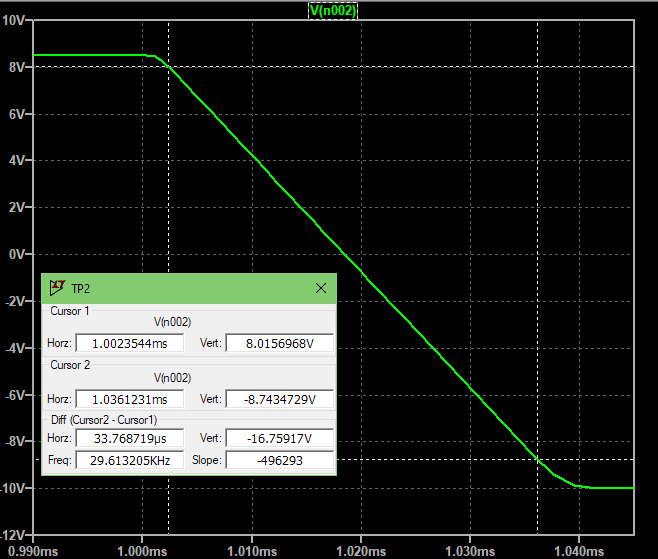
\includegraphics[height=5cm]{Imágenes/Simulaciones/SR 50ohm.jpeg}
    	\caption{Pendiente de Slew Rate}
    \end{figure} 
    \centerline{\textbf{SR=0,496V/uS}
    }
    
\section{Caso de Estudio:$R_{i} = 100 K\Omega$ }
Ahora para este caso, se tiene una fuente con una impedancia de entrada muy mayor, por lo cual, será más difícil la implementación sin perturbar la señal de entrada, para ello, tomamos al igual que en el anterior análisis:\\

$R_{i} = 100 [K\Omega] \xrightarrow{} Z_{i1,2} \ge 10*R_{i} $\\

$R \ge 1[M\Omega] $\\

Si tomo que $R=1.8 [M\Omega]$, entonces:

$\frac{R_{f}}{R} = 30 \xrightarrow{} R_{f} = 54 [M\Omega]$.\\

Como vemos, esto no cumple con la especificación dada que $R_f$ no debe superar los $10 [M\Omega]$, por lo cual se agregará una red tipo T tal que se cumpla con lo especificado.\\

Supongo la entrada inversora pasivada, por lo cual:\\

$i_f = \frac{V_o}{R_2 + R_1//R_3}* R_1//R_3 * \frac{1}{R_1}$\\

$\frac{V_o}{i_f} = \frac{R_2*R_1}{R_3} + R_2 + R_1 = R_f$\\

Sii tomo $R_1 = R_2 = 220 [K\Omega]$.\\

\begin{center}
    \boxed{R_3 = 903.66 [\Omega]}
\end{center}

De esta manera podemos lograr el requerimiento.\\

\subsection{Errores DC}
Incorporar la red T, hace que la ganancia de lazo ahora esté determinada por la siguiente expresión:\\

\begin{center}
    \boxed{T = -\frac{1}{2} * \frac{Ad*R*R_3}{ (R_1 + R/2) * (R_2 + R_3)} = 328.72}
\end{center}

En este caso no volvemos a simular el Error de Vos ya que resultaria el mismo que en el caso anterior.
\begin{itemize}

    \item $\Delta V_{o}|_{vos} = (1 + 2*\frac{R_f}{R})*V_{os} = 36.6 [mV].$
    \item $\Delta V_{o}|_{Ios} = I_{os}.R_f = 540 [mV].$
    \begin{figure}[H]
    \centering
    \begin{minipage}{0.48\textwidth}
        \centering
        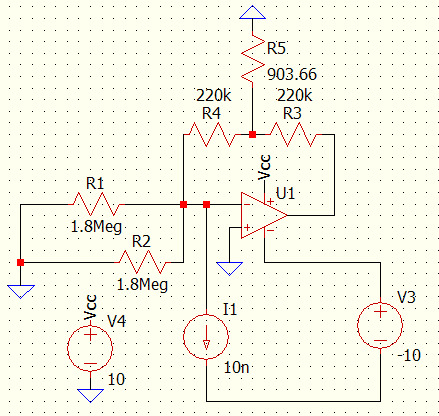
\includegraphics[height=5cm]{Imágenes/Simulaciones/ios diagrama.jpeg}
        \caption{Diagrama de Error Ios.}
        \label{fig:diagrama_vos}
    \end{minipage}
    \hfill
    \begin{minipage}{0.48\textwidth}
        \centering
        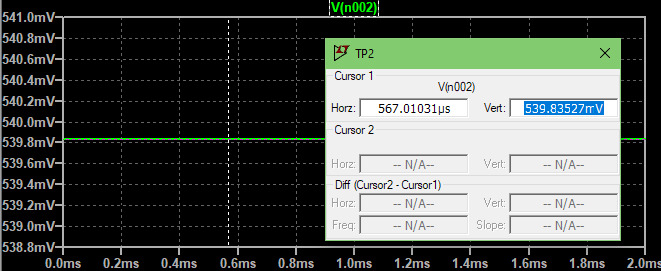
\includegraphics[height=5cm, width=8cm]{Imágenes/Simulaciones/ios 100.jpeg}
        \caption{Simulación del Error Ios.}
        \label{fig:simu_vos}
    \end{minipage}
\end{figure}
    \item $\Delta V_{o}|_{Ad < \infty} = \frac{FS}{To} = 30.421 [mV].$
    \item $\Delta V_{o}|_{RRMC < \infty} = 0 [mV].$
\end{itemize}

Por lo que el error total en contínua será de $\Delta Vo = 0.607 [V].$, por lo que se ve, se debería agregar una etapa anterior como adaptación de impredancia, tal como un \textbf{buffer de tensión}.\\

\subsection{Errores AC}
\textbf{Ancho de Banda de plena Potencia}.\\

$f_{HP} = \frac{SR}{2*\pi*V_{pp}} = 8 [KHz].$\\

\textbf{Ancho de Banda de pequeña Señal}.\\

$f_{HP} = k.f_T = 3.28 [KHz]$\\
\begin{figure}[H]
    	\centering
    	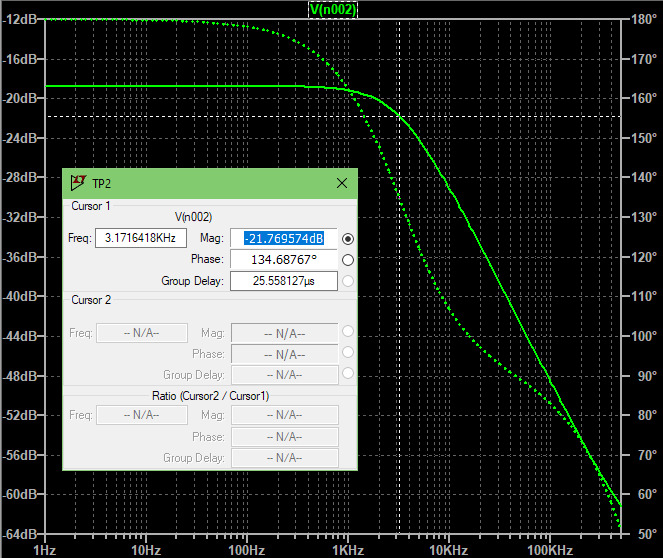
\includegraphics[height=5cm]{Imágenes/Simulaciones/bode 100.jpeg}
    	\caption{Diagrama de Bode Pequeña Señal}
    \end{figure}
\newpage
\textbf{Error Vectorial}.\\

    \begin{figure}[ht]
    	\centering
    	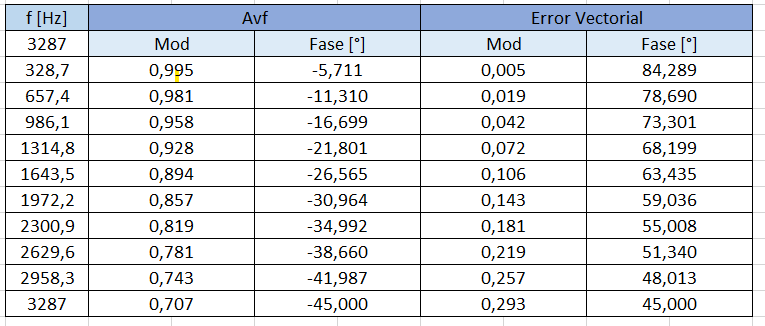
\includegraphics[height=5cm]{Imágenes/err2.png}
    	\caption{Error Vectorial}
    \end{figure}

